\documentclass[a4paper]{article}

%% Language and font encodings
\usepackage[english]{babel}
\usepackage[utf8]{inputenc}
\usepackage[T1]{fontenc}

%% Sets page size and margins
\usepackage[a4paper,top=3cm,bottom=2cm,left=3cm,right=3cm,marginparwidth=1.75cm]{geometry}

%% Useful packages
\usepackage{amsmath}

\usepackage{graphicx}
\usepackage{listings}
\graphicspath{{./images/}}
\usepackage{tikz}
\usetikzlibrary{arrows}
\usepackage[style=numeric]{biblatex}
\usepackage{enumitem}
\setlist[description]{leftmargin=\parindent,labelindent=\parindent}

\addbibresource{template_Report.bib}


\usepackage[colorinlistoftodos]{todonotes}
\usepackage[colorlinks=true, allcolors=blue]{hyperref}
\usepackage{xfrac}

\title{\textbf{Simple SIMD Programming Example}\\CompMeth Spring 2018}

\author{Davide Pola}

\begin{document}
\maketitle

\tableofcontents

\section{Introduction}

The goal of this report is to illustrate the work done on computing fixed point multiplications in C with and without the SIMD ISA extension from Intel. The work have been entirely developed for the CompMeth course in EURECOM.

\subsection{Content}
First of all, a small introducing section will generally speak about SIMD and show a very simple example of a SIMD instruction.
Later, Sections \ref{real} and \ref{complex} will separately cover real and complex fixed point multiplication, with a focus on the developed code.
Section \ref{setup} covers in detail all the setup required to obtain valuable results and finally Section \ref{results} consist of visualization and comments about the simulations.

\section{SIMD}\label{intro}
\subsection{SIMD support}
Most recent high-end CPUs support SIMD, which stands for \textbf{S}ingle \textbf{I}nstruction \textbf{M}ultiple \textbf{D}ata. These kind of instructions are specifically targeted to exploit data level parallelism in order to improve performance for specific tasks, such as image and signal processing or scientific calculus.
\\\\Every recent CPU architecture has his own SIMD instruction set: 
\begin{description}
	\item[Intel] - MMX, SSE, AVX, AVX2
	\item[AMD] - 3DNow!, SSE, AVX, AVX2
	\item[ARM] - NEON
\end{description}
In order to discover which SIMD extensions are enabled on a given CPU, either refer to the Product Specification, or issue the command \lstinline[language=bash, basicstyle=\ttfamily]{grep flags /proc/cpuinfo} (on Linux).
As the target CPU used in this project is an Intel i7-4510u, all possible informations can be found in \autocite{4510u}

\subsection{How to code with SIMD}
There are 4 different ways to code using SIMD:
\begin{itemize}
	\item SIMD enabled libraries
	\item Compiler auto-vectorization
	\item SIMD Intrinsics
	\item SIMD Assembly Code
\end{itemize}
In this work, most of the code is developed with Intel SSE/AVX Intrinsics as the target machine is a Haswell equipped laptop. Unfortunately, there is no support for AVX-512 extension as it is recent and at the moment of writing (Q2 2018) only targeted to HPC and high-end processors.

\subsection{Example of an SIMD Instruction}
A regular CPU operates on scalars, one at a time. A vector processor, on the other hand, lines up a whole row of these scalars, all of the same type, and operates on them as a unit. Here is an example that will help to understand a little the SIMD instructions. Figure \ref{fig:PADD} shows a simple scheme of the PADDD instruction (SSE2).
\begin{figure}[h]
	\centering
	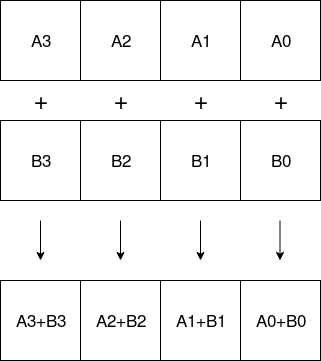
\includegraphics[width=.4\linewidth]{sse_add.png}
	\caption{SSE PADDD scheme.}
	\label{fig:PADD}
\end{figure}
\\The PADDD mnemonic means packed addition for double-word. This assembly instruction receives two 128-bit input parameters that contain four 32-bit integers each. The instruction returns a 128-bit output that contains the sum for each of the four 32-bit integers, packed in the 128-bit output. You can calculate the sum for four 32-bit signed integers with a single call to the PADDD instruction. If you have to calculate the sum for 100 couples of 32-bit integers, you can do it with 25 calls to this instruction instead of using a single instruction for each couple. It is possible to achieve very important speedups. However, because it is sometimes necessary to pack the data before calling the SIMD instruction and then unpack the output, it is also important to measure this overhead that adds some code.

\section{Real Fixed Point Multiplication} \label{real}
\subsection{Scalar}
The scalar operation required is quite simple. Two 16-bit numbers (internally Q1.15) need to be multiplied, this is done simply by multiplying them as standard unsigned 32 bits, then shift right the outcome of 15 positions (16-1 because the sign would be on the two most significant bits). Only the lowest 16 bits will remain after the last typecasting to 16-bit.
This operation is then repeated in a \lstinline[language=c, basicstyle=\ttfamily]{for} loop for each element that needs to be computed.

\begin{lstlisting}[language=c,frame=tb,caption=Scalar Real Fixed Point Multiplication]
for(i=0;i<N;i++){
  z[i] = (uint16_t) ((((uint32_t) x[i]) * y[i]) >> 15);
  }
\end{lstlisting}

\subsection{SIMD}
In the SIMD case, the operation is split in chunks of 8 (SSE) or 16 (AVX) integers operated in parallel. The surrounding loop is then iterating on \sfrac{1}{8} or \sfrac{1}{16} of the previous N.

\begin{lstlisting}[language=c,frame=tb,caption=AVX2 Real Fixed Point Multiplication,label=realSIMD]
__m256i *x256 = (__m256i *)x;
__m256i *y256 = (__m256i *)y;
__m256i *z256 = (__m256i *)z;

uint32_t i;

N>>=4;
for(i=0; i<N; i++)
{   
	z256[i] = _mm256_mulhrs_epi16(x256[i], y256[i]);
}
\end{lstlisting}

Fortunately, both SSE and AVX extension provide an intrinsic which is perfectly shaped for this purpose:
\begin{description}
	\item[AVX2] \lstinline[language=c, basicstyle=\ttfamily]{__m256i _mm256_mulhrs_epi16 (__m256i a, __m256i b)}
	\item[SSE3] \lstinline[language=c, basicstyle=\ttfamily]{__m128i _mm_mulhrs_epi16 (__m128i a, __m128i b)}
\end{description}
As can be seen in Listing \ref{realSIMD}, the arrays coming need first to be typecasted to the intrinsic variable, then the process could be done. Please note that no packing and unpacking is required as the numbers are already distributed in the correct way (alignment problems will be discussed later).
 
\section{Complex Fixed Point Multiplication} \label{complex}
The first problem related to complex multiplication is due to the representation of numbers. They can be either placed in a structure, thus in an interleaved real/imaginary fashion, or have two separate arrays for reals and imaginaries, both the two cases have been treated in this work.

\subsection{Interleaved fashion}
The basic structure of a complex number is defined in C as follows:
\begin{lstlisting}[language=c,frame=tb,caption=Complex Number Structure,label=complex16]
typedef struct complex16 { 
int16_t r;                   
int16_t i;                   
} complex16;    
\end{lstlisting}

\subsubsection{Scalar}

Again, the scalar code is pretty straightforward, the code can be seen in Listing \ref{complexScalar}.
\begin{lstlisting}[language=c,frame=tb,caption=Scalar Complex Fixed Point Multiplication - Interleaved Fashion,label=complexScalar]
for(i=0;i<N;i++){    
  z[i].r = (uint16_t) ((((int32_t) x[i].r) * ((int32_t)y[i].r) -
                        ((int32_t) x[i].i) * ((int32_t) y[i].i)) >> 15);
  z[i].i = (uint16_t) ((((int32_t) x[i].r) * ((int32_t)y[i].i) +
                        ((int32_t) x[i].i) * ((int32_t) y[i].r)) >> 15);
  }
\end{lstlisting}

\subsubsection{SIMD}
Here is where the thing becomes a little complicated. Neither SSE nor AVX extension implement function to immediately perform this operation on fixed point representation (they have FMADD but only in floating point). It is then necessary to create a small algorithm that generates the correct output using intrinsics.
\\Another important aspect to remember is endianess: Intel CPUs operate in Little-Endian, this means that lower addresses correspond to lower significant bits. As an example, in a SSE 128-bit register, the 4 16-bit fixed point numbers it contains will be distributed as depicted in Figure \ref{fig:endianess}. It is then important to know that data is received in this format and that the output needs to be coherent with it.
\begin{figure}[h]
	\centering
	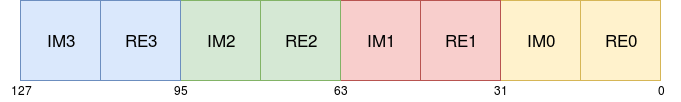
\includegraphics[width=\linewidth]{endianess.png}
	\caption{Endianess Example - 4 16-bit Complex Numbers Represented on 128 bits.}
	\label{fig:endianess}
\end{figure}
\\The algorithm is the following:
\begin{description}
	\item[sign :]  negate imaginary parts of b
    \item[madd :] multiply and add for real part
    \item[srli :] shift real parts right to LSB
	\item[shuffle :] swap adjacent pairs of c and d in order to have columns aligned for the next operation
	\item[madd :] multiply and add for imaginary part
	\item[slli :] just erase double sign bit from imaginary part, result is already in MSB
	\item[blend :] create the final result merging the two vectors 
\end{description}
For further explanations regarding the exact operations performed by the intrinsics, please refer to \autocite{IIG}. 

\begin{lstlisting}[language=c,frame=tb,caption=AVX2 Complex Fixed Point Multiplication - Interleaved Fashion,label=complexSIMD]
static inline void componentwise_multiply_complex_struct_avx2(
complex16 *x,complex16 *y, complex16 *z, int N){
__m256i *x256 = (__m256i *)x;
__m256i *y256 = (__m256i *)y;
__m256i *z256 = (__m256i *)z;
__m256i const perm_mask=_mm256_set_epi8(
29,28,31,30,25,24,27,26,21,20,23,22,17,16,19,18,
13,12,15,14, 9, 8,11,10, 5, 4, 7, 6, 1, 0, 3, 2);
register __m256i mmtmpb_real;
register __m256i mmtmpb_imag;

int i;
N>>=4;
for(i=0; i<N; i++)
{
  mmtmpb_real    = _mm256_sign_epi16(y256[i],*(__m256i*)reflip_256);
  mmtmpb_real    = _mm256_madd_epi16(x256[i],mmtmpb_real);
  mmtmpb_real    = _mm256_srli_epi32(mmtmpb_real, 15);

  mmtmpb_imag    = _mm256_shuffle_epi8(y256[i],perm_mask);
  mmtmpb_imag    = _mm256_madd_epi16(x256[i],mmtmpb_imag);
  mmtmpb_imag    =_mm256_slli_epi32 (mmtmpb_imag, 1);

  z256[i] = _mm256_blend_epi16(mmtmpb_imag,mmtmpb_real,0xAA);
}
\end{lstlisting}

\subsection{Separated Array Fashion}
As already introduced, complex number could be also treated with separated real and complex parts. The functions developed here thus have 4 input arrays instead of 2: a couple for each operand. Obviously output is on two vectors too, one for real and the other for complex.
\\Actually, due to this particular aspect, the amount of data operated in each iteration is the double than in the other cases, however the total amount of data processed is the same, as the input vectors are half the length of the others.

\subsubsection{Scalar}
The scalar approach is again straightforward. The code is identical to Listing \ref{complexScalar} with the exception that now each vector is indexed separately.
\begin{lstlisting}[language=c,frame=tb,caption=Scalar Complex Fixed Point Multiplication - Separeted Array Fashion,label=complexScalarArray]
for(i=0;i<N;i++){    
  x[i] = (uint16_t) ((((int32_t) a[i]) * ((int32_t) c[i]) -
                      ((int32_t) b[i]) * ((int32_t) d[i])) >> 15);
  y[i] = (uint16_t) ((((int32_t) a[i]) * ((int32_t) d[i]) +
                      ((int32_t) b[i]) * ((int32_t) c[i])) >> 15);	
}
\end{lstlisting} 

\subsubsection{SIMD}
Unlike the previous case, here there is no problem related to endianess and data representation, as no structure is involved. However, there is not an instruction able to perform both multiplication and addition at the same time. This means that the two operations need to be performed separately.
\\\\The algorithm is pretty simple, first compute the 4 required multiplication and later perform the addition (or subtraction) of the previously computed couples. The resulting code (AVX) can be seen in Listing \ref{complexSIMDArray}.
\begin{lstlisting}[language=c,frame=tb,caption=AVX2 Complex Fixed Point Multiplication - Separated Array Fashion,label=complexSIMDArray]
for(i=0; i<N; i++){ 
  ac256 = _mm256_mulhrs_epi16(a256[i], c256[i]); 
  bc256 = _mm256_mulhrs_epi16(b256[i], c256[i]); 
  bd256 = _mm256_mulhrs_epi16(b256[i], d256[i]); 
  ad256 = _mm256_mulhrs_epi16(a256[i], d256[i]); 

  x256[i] = _mm256_sub_epi16(ac256,bd256); 
  y256[i] = _mm256_add_epi16(bc256,ad256); 
} 
\end{lstlisting}

\section{Simulation Setup and Timing Problems} \label{setup}
\subsection{Alignment}
Alignment is very important for SIMD functions: having unaligned data often causes a strong performance degradation (two memory accesses are required instead of one), also, the compiler will struggle to compile SIMD intrinsics if the memory is not guaranteed to be aligned.
\\Two solutions are possible for this problem, both equivalent:
\begin{itemize}
	\item append \lstinline[language=c, basicstyle=\ttfamily]{__attribute__((aligned(n)))} compiler directive after memory pointers declarations
	\item use an allocating function able to handle alignment, such as \lstinline[language=c, basicstyle=\ttfamily]{aligned_alloc(n,size)}
\end{itemize}

\subsection{Compiler optimizations} \label{setup-comp}

GCC is the compiler used for this entire project, it supports 6 optimization levels, if you need further information, please refer to \autocite{GCCOPT}.

The targets of this experiments are O0, O2 and O3 (O1 is very little used).
\begin{description}
	\item[O0:] no optimization, all the code is traduced almost 1:1 by the compiler. This is the less efficient choice
	\item[O2:] enable all optimizations but those that require space/performance trade-off
	\item[O3:] same as O2 but focus on performance and usually enable optimizations that increase the size of the code
\end{description}
One of the optimizations we care much about is \textbf{auto-vectorization}: with this feature, the compiler is able to automatically detect parts of the code that could been improved by exploiting SIMD hardware, thus the programmer no more needs to write complex SIMD code. This feature is enabled by default in O3.
\\Unfortunately, by default, the compiler can not make strong assumptions on the data to be processed, and cannot produce a perfect result.
The solution is to give "hints" to the compiler in order to exploit maximum optimization.
\\One example of this behavior is pointer aliasing, very well explained in \autocite{ALIAS}.
By setting the restrict keyword to parameters in functions declarations, the compiler is able to freely reorder and vectorize loops, leading to better performance.(the very same behavior can be achieved by setting \lstinline[language=c, basicstyle=\ttfamily]{#pragma GCC ivdep} just before the loop)

\subsection{Accurate timing vs operating system}
The worst enemy of profilers is for sure the operating system. The OS can cause a lot of nondeterministic overhead to the program due to preemption and context switch, also altering cache and branch predictor status. Multicore processors suffer less from this particular aspect as in general there is less contention on a given core, thus the user application \textit{should} be given more freedom to run.
\\However, to achieve the best results out of the test machine, something more sophisticated can be done.
Linux kernel provides a nice feature called \textbf{isolation}: it is possible to avoid any application to run on one (or more) CPU of the system with the \lstinline[language=c, basicstyle=\ttfamily]{isolcpus} directive, more information about it could be found in \autocite{ISOLCPU}.
The running CPU is a quad core system, core 3 was isolated from the rest.
\\ After doing this, complete real time is still not guaranteed, it is necessary to set the program as the maximum possible priority. By default Linux uses CFS (Completely Fair Scheduler) that, among the others, implements a FIFO real-time scheduling policy \autocite{SCHEDU}. 
By setting the code in Listing \ref{sched} at the beginning of the C program, it will change itself to the FIFO policy with the maximum priority (99), this will make its execution uninterruptible (to be verified). (be careful, this locks the entire OS until the program is terminates its execution)

\begin{lstlisting}[language=c,frame=tb,caption=Scheduler Policy Change,label=sched]
struct sched_param param;
param.sched_priority = 99;
if (sched_setscheduler(0, SCHED_FIFO, & param) != 0) {
  perror("sched_setscheduler");
  exit(EXIT_FAILURE);  
  }
\end{lstlisting}

\subsection{Performance counters}
Precise clock cycles count can be achieved by reading the performance counters provided by the CPU. The time measured by TSC (accessible with \lstinline[language=c, basicstyle=\ttfamily]{rdtsc} function) is not exactly cpu clocks, at least not in Haswell CPUs (in general in all those that support DVFS), but CPU clocks referred to a fixed frequency, regardless the actual frequency of the processor. More information related to TSC can be found in \autocite{TSC}.
\\In order to pursuit the best possible cycle count accuracy, an additional library has been used, named \textbf{libpfc}. This custom library provides an useful and simple API to the programmer in order to use all the performance counters provided by the CPU, including the variant TSC.(many other possible profiling can be measured, such as issued instructions or cache misses). More information and the installing tutorial can be found in \autocite{LIBPFC}.

\section{Simulation results} \label{results}
\begin{figure}[ht!]
	\centering
	\resizebox{1.0\textwidth}{!}{% GNUPLOT: LaTeX picture with Postscript
\begingroup
  \makeatletter
  \providecommand\color[2][]{%
    \GenericError{(gnuplot) \space\space\space\@spaces}{%
      Package color not loaded in conjunction with
      terminal option `colourtext'%
    }{See the gnuplot documentation for explanation.%
    }{Either use 'blacktext' in gnuplot or load the package
      color.sty in LaTeX.}%
    \renewcommand\color[2][]{}%
  }%
  \providecommand\includegraphics[2][]{%
    \GenericError{(gnuplot) \space\space\space\@spaces}{%
      Package graphicx or graphics not loaded%
    }{See the gnuplot documentation for explanation.%
    }{The gnuplot epslatex terminal needs graphicx.sty or graphics.sty.}%
    \renewcommand\includegraphics[2][]{}%
  }%
  \providecommand\rotatebox[2]{#2}%
  \@ifundefined{ifGPcolor}{%
    \newif\ifGPcolor
    \GPcolortrue
  }{}%
  \@ifundefined{ifGPblacktext}{%
    \newif\ifGPblacktext
    \GPblacktextfalse
  }{}%
  % define a \g@addto@macro without @ in the name:
  \let\gplgaddtomacro\g@addto@macro
  % define empty templates for all commands taking text:
  \gdef\gplbacktext{}%
  \gdef\gplfronttext{}%
  \makeatother
  \ifGPblacktext
    % no textcolor at all
    \def\colorrgb#1{}%
    \def\colorgray#1{}%
  \else
    % gray or color?
    \ifGPcolor
      \def\colorrgb#1{\color[rgb]{#1}}%
      \def\colorgray#1{\color[gray]{#1}}%
      \expandafter\def\csname LTw\endcsname{\color{white}}%
      \expandafter\def\csname LTb\endcsname{\color{black}}%
      \expandafter\def\csname LTa\endcsname{\color{black}}%
      \expandafter\def\csname LT0\endcsname{\color[rgb]{1,0,0}}%
      \expandafter\def\csname LT1\endcsname{\color[rgb]{0,1,0}}%
      \expandafter\def\csname LT2\endcsname{\color[rgb]{0,0,1}}%
      \expandafter\def\csname LT3\endcsname{\color[rgb]{1,0,1}}%
      \expandafter\def\csname LT4\endcsname{\color[rgb]{0,1,1}}%
      \expandafter\def\csname LT5\endcsname{\color[rgb]{1,1,0}}%
      \expandafter\def\csname LT6\endcsname{\color[rgb]{0,0,0}}%
      \expandafter\def\csname LT7\endcsname{\color[rgb]{1,0.3,0}}%
      \expandafter\def\csname LT8\endcsname{\color[rgb]{0.5,0.5,0.5}}%
    \else
      % gray
      \def\colorrgb#1{\color{black}}%
      \def\colorgray#1{\color[gray]{#1}}%
      \expandafter\def\csname LTw\endcsname{\color{white}}%
      \expandafter\def\csname LTb\endcsname{\color{black}}%
      \expandafter\def\csname LTa\endcsname{\color{black}}%
      \expandafter\def\csname LT0\endcsname{\color{black}}%
      \expandafter\def\csname LT1\endcsname{\color{black}}%
      \expandafter\def\csname LT2\endcsname{\color{black}}%
      \expandafter\def\csname LT3\endcsname{\color{black}}%
      \expandafter\def\csname LT4\endcsname{\color{black}}%
      \expandafter\def\csname LT5\endcsname{\color{black}}%
      \expandafter\def\csname LT6\endcsname{\color{black}}%
      \expandafter\def\csname LT7\endcsname{\color{black}}%
      \expandafter\def\csname LT8\endcsname{\color{black}}%
    \fi
  \fi
    \setlength{\unitlength}{0.0500bp}%
    \ifx\gptboxheight\undefined%
      \newlength{\gptboxheight}%
      \newlength{\gptboxwidth}%
      \newsavebox{\gptboxtext}%
    \fi%
    \setlength{\fboxrule}{0.5pt}%
    \setlength{\fboxsep}{1pt}%
\begin{picture}(10080.00,7544.00)%
    \gplgaddtomacro\gplbacktext{%
      \csname LTb\endcsname%
      \put(396,924){\makebox(0,0)[r]{\strut{}\LARGE{$10^{1}$}}}%
      \csname LTb\endcsname%
      \put(396,2094){\makebox(0,0)[r]{\strut{}\LARGE{$10^{2}$}}}%
      \csname LTb\endcsname%
      \put(396,3264){\makebox(0,0)[r]{\strut{}\LARGE{$10^{3}$}}}%
      \csname LTb\endcsname%
      \put(396,4433){\makebox(0,0)[r]{\strut{}\LARGE{$10^{4}$}}}%
      \csname LTb\endcsname%
      \put(396,5603){\makebox(0,0)[r]{\strut{}\LARGE{$10^{5}$}}}%
      \csname LTb\endcsname%
      \put(396,6773){\makebox(0,0)[r]{\strut{}\LARGE{$10^{6}$}}}%
      \csname LTb\endcsname%
      \put(528,594){\makebox(0,0){\strut{}\LARGE{$0$}}}%
      \csname LTb\endcsname%
      \put(1639,594){\makebox(0,0){\strut{}\LARGE{$1024$}}}%
      \csname LTb\endcsname%
      \put(2749,594){\makebox(0,0){\strut{}\LARGE{$2048$}}}%
      \csname LTb\endcsname%
      \put(3860,594){\makebox(0,0){\strut{}\LARGE{$3072$}}}%
      \csname LTb\endcsname%
      \put(4970,594){\makebox(0,0){\strut{}\LARGE{$4096$}}}%
      \csname LTb\endcsname%
      \put(6081,594){\makebox(0,0){\strut{}\LARGE{$5120$}}}%
      \csname LTb\endcsname%
      \put(7191,594){\makebox(0,0){\strut{}\LARGE{$6144$}}}%
      \csname LTb\endcsname%
      \put(8302,594){\makebox(0,0){\strut{}\LARGE{$7168$}}}%
      \csname LTb\endcsname%
      \put(9412,594){\makebox(0,0){\strut{}\LARGE{$8192$}}}%
    }%
    \gplgaddtomacro\gplfronttext{%
      \csname LTb\endcsname%
      \put(-374,3848){\rotatebox{-270}{\makebox(0,0){\strut{}\LARGE{clock cycles}}}}%
      \put(5039,154){\makebox(0,0){\strut{}\LARGE{input size [bytes]}}}%
      \put(5039,7213){\makebox(0,0){\strut{}\Large{\shortstack{ Scalar vs Intrinsics Compilation on 16-bit Fixed Point Complex Multiplication\\ Average on 500000 iterations}}}}%
      \csname LTb\endcsname%
      \put(8564,2197){\makebox(0,0)[r]{\strut{}\normalsize{O0 SCALAR CMPLX STRUCT}}}%
      \csname LTb\endcsname%
      \put(8564,1977){\makebox(0,0)[r]{\strut{}\normalsize{O0 AVX2 CMPLX STRUCT}}}%
      \csname LTb\endcsname%
      \put(8564,1757){\makebox(0,0)[r]{\strut{}\normalsize{O2 SCALAR CMPLX STRUCT}}}%
      \csname LTb\endcsname%
      \put(8564,1537){\makebox(0,0)[r]{\strut{}\normalsize{O2 AVX2 CMPLX STRUCT}}}%
      \csname LTb\endcsname%
      \put(8564,1317){\makebox(0,0)[r]{\strut{}\normalsize{O3 SCALAR CMPLX STRUCT}}}%
      \csname LTb\endcsname%
      \put(8564,1097){\makebox(0,0)[r]{\strut{}\normalsize{O3 AVX2 CMPLX STRUCT}}}%
    }%
    \gplbacktext
    \put(0,0){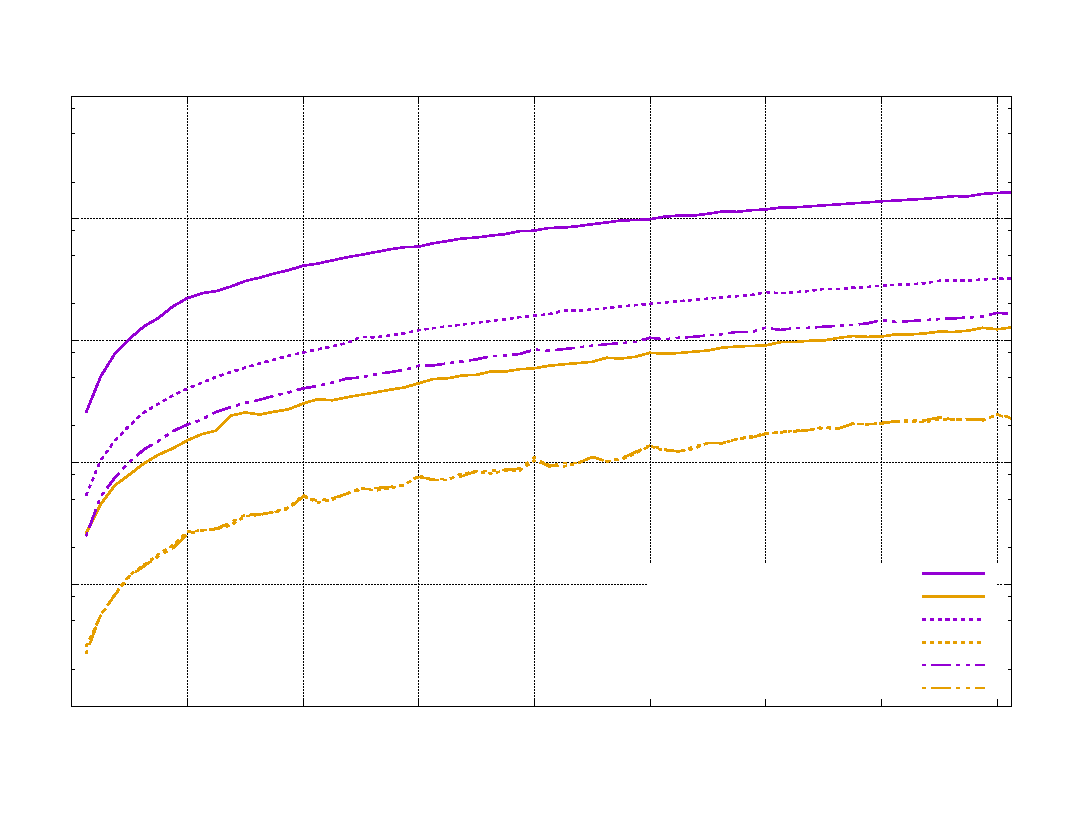
\includegraphics{optim}}%
    \gplfronttext
  \end{picture}%
\endgroup
}
	\caption{Input dynamic range calculation.}
	\label{Fig:OPTIM}
\end{figure}
First of all, it is interesting to see the performance change at various compiler optimization levels of SIMD intrinsics coding against a standard scalar approach. According to Figure \ref{Fig:OPTIM}, SIMD intrinsics perform always better at any optimization level for complex "struct" multiplication, similar results have been achieved for the others multiplications.
\\\\Other than that, another important evaluation needs to be performed: How do the various SIMD and scalar functions perform at different optimization levels?
Figure \ref{Fig:SCALAR} shows this information for what concerns the real multiplication.
For what concerns SIMD intrinsics (orange and light-blue lines), there is approximately no difference between O2 and O3, while there is a huge gap in the scalar counterpart. This is very likely due to auto-vectorization as previously mentioned in Section \ref{setup-comp}. By comparing the disassembled code (not provided here) between O2 and O3, this phenomena is very clear: the multiplication loop has been completely vectorized (a confirmation of this comes from the log produced by \lstinline[language=c, basicstyle=\ttfamily]{-fopt-info-vect} option passed to GCC).
\begin{figure}
	\centering
	\resizebox{1.0\textwidth}{!}{% GNUPLOT: LaTeX picture with Postscript
\begingroup
  \makeatletter
  \providecommand\color[2][]{%
    \GenericError{(gnuplot) \space\space\space\@spaces}{%
      Package color not loaded in conjunction with
      terminal option `colourtext'%
    }{See the gnuplot documentation for explanation.%
    }{Either use 'blacktext' in gnuplot or load the package
      color.sty in LaTeX.}%
    \renewcommand\color[2][]{}%
  }%
  \providecommand\includegraphics[2][]{%
    \GenericError{(gnuplot) \space\space\space\@spaces}{%
      Package graphicx or graphics not loaded%
    }{See the gnuplot documentation for explanation.%
    }{The gnuplot epslatex terminal needs graphicx.sty or graphics.sty.}%
    \renewcommand\includegraphics[2][]{}%
  }%
  \providecommand\rotatebox[2]{#2}%
  \@ifundefined{ifGPcolor}{%
    \newif\ifGPcolor
    \GPcolortrue
  }{}%
  \@ifundefined{ifGPblacktext}{%
    \newif\ifGPblacktext
    \GPblacktextfalse
  }{}%
  % define a \g@addto@macro without @ in the name:
  \let\gplgaddtomacro\g@addto@macro
  % define empty templates for all commands taking text:
  \gdef\gplbacktext{}%
  \gdef\gplfronttext{}%
  \makeatother
  \ifGPblacktext
    % no textcolor at all
    \def\colorrgb#1{}%
    \def\colorgray#1{}%
  \else
    % gray or color?
    \ifGPcolor
      \def\colorrgb#1{\color[rgb]{#1}}%
      \def\colorgray#1{\color[gray]{#1}}%
      \expandafter\def\csname LTw\endcsname{\color{white}}%
      \expandafter\def\csname LTb\endcsname{\color{black}}%
      \expandafter\def\csname LTa\endcsname{\color{black}}%
      \expandafter\def\csname LT0\endcsname{\color[rgb]{1,0,0}}%
      \expandafter\def\csname LT1\endcsname{\color[rgb]{0,1,0}}%
      \expandafter\def\csname LT2\endcsname{\color[rgb]{0,0,1}}%
      \expandafter\def\csname LT3\endcsname{\color[rgb]{1,0,1}}%
      \expandafter\def\csname LT4\endcsname{\color[rgb]{0,1,1}}%
      \expandafter\def\csname LT5\endcsname{\color[rgb]{1,1,0}}%
      \expandafter\def\csname LT6\endcsname{\color[rgb]{0,0,0}}%
      \expandafter\def\csname LT7\endcsname{\color[rgb]{1,0.3,0}}%
      \expandafter\def\csname LT8\endcsname{\color[rgb]{0.5,0.5,0.5}}%
    \else
      % gray
      \def\colorrgb#1{\color{black}}%
      \def\colorgray#1{\color[gray]{#1}}%
      \expandafter\def\csname LTw\endcsname{\color{white}}%
      \expandafter\def\csname LTb\endcsname{\color{black}}%
      \expandafter\def\csname LTa\endcsname{\color{black}}%
      \expandafter\def\csname LT0\endcsname{\color{black}}%
      \expandafter\def\csname LT1\endcsname{\color{black}}%
      \expandafter\def\csname LT2\endcsname{\color{black}}%
      \expandafter\def\csname LT3\endcsname{\color{black}}%
      \expandafter\def\csname LT4\endcsname{\color{black}}%
      \expandafter\def\csname LT5\endcsname{\color{black}}%
      \expandafter\def\csname LT6\endcsname{\color{black}}%
      \expandafter\def\csname LT7\endcsname{\color{black}}%
      \expandafter\def\csname LT8\endcsname{\color{black}}%
    \fi
  \fi
    \setlength{\unitlength}{0.0500bp}%
    \ifx\gptboxheight\undefined%
      \newlength{\gptboxheight}%
      \newlength{\gptboxwidth}%
      \newsavebox{\gptboxtext}%
    \fi%
    \setlength{\fboxrule}{0.5pt}%
    \setlength{\fboxsep}{1pt}%
\begin{picture}(10080.00,7544.00)%
    \gplgaddtomacro\gplbacktext{%
      \csname LTb\endcsname%
      \put(396,924){\makebox(0,0)[r]{\strut{}\LARGE{$10^{1}$}}}%
      \csname LTb\endcsname%
      \put(396,2386){\makebox(0,0)[r]{\strut{}\LARGE{$10^{2}$}}}%
      \csname LTb\endcsname%
      \put(396,3849){\makebox(0,0)[r]{\strut{}\LARGE{$10^{3}$}}}%
      \csname LTb\endcsname%
      \put(396,5311){\makebox(0,0)[r]{\strut{}\LARGE{$10^{4}$}}}%
      \csname LTb\endcsname%
      \put(396,6773){\makebox(0,0)[r]{\strut{}\LARGE{$10^{5}$}}}%
      \csname LTb\endcsname%
      \put(528,594){\makebox(0,0){\strut{}\LARGE{$0$}}}%
      \csname LTb\endcsname%
      \put(1639,594){\makebox(0,0){\strut{}\LARGE{$1024$}}}%
      \csname LTb\endcsname%
      \put(2749,594){\makebox(0,0){\strut{}\LARGE{$2048$}}}%
      \csname LTb\endcsname%
      \put(3860,594){\makebox(0,0){\strut{}\LARGE{$3072$}}}%
      \csname LTb\endcsname%
      \put(4970,594){\makebox(0,0){\strut{}\LARGE{$4096$}}}%
      \csname LTb\endcsname%
      \put(6081,594){\makebox(0,0){\strut{}\LARGE{$5120$}}}%
      \csname LTb\endcsname%
      \put(7191,594){\makebox(0,0){\strut{}\LARGE{$6144$}}}%
      \csname LTb\endcsname%
      \put(8302,594){\makebox(0,0){\strut{}\LARGE{$7168$}}}%
      \csname LTb\endcsname%
      \put(9412,594){\makebox(0,0){\strut{}\LARGE{$8192$}}}%
    }%
    \gplgaddtomacro\gplfronttext{%
      \csname LTb\endcsname%
      \put(-374,3848){\rotatebox{-270}{\makebox(0,0){\strut{}\LARGE{clock cycles}}}}%
      \put(5039,154){\makebox(0,0){\strut{}\LARGE{input size [bytes]}}}%
      \put(5039,7213){\makebox(0,0){\strut{}\Large{\shortstack{Compiler Comparison on 16-bit Fixed Point Real Multiplication\\ Average on 500000 iterations}}}}%
      \csname LTb\endcsname%
      \put(8564,2857){\makebox(0,0)[r]{\strut{}\normalsize{O0 SCALAR REAL}}}%
      \csname LTb\endcsname%
      \put(8564,2637){\makebox(0,0)[r]{\strut{}\normalsize{O0 SSE4 REAL}}}%
      \csname LTb\endcsname%
      \put(8564,2417){\makebox(0,0)[r]{\strut{}\normalsize{O0 AVX2 REAL}}}%
      \csname LTb\endcsname%
      \put(8564,2197){\makebox(0,0)[r]{\strut{}\normalsize{O2 SCALAR REAL}}}%
      \csname LTb\endcsname%
      \put(8564,1977){\makebox(0,0)[r]{\strut{}\normalsize{O2 SSE4 REAL}}}%
      \csname LTb\endcsname%
      \put(8564,1757){\makebox(0,0)[r]{\strut{}\normalsize{O2 AVX2 REAL}}}%
      \csname LTb\endcsname%
      \put(8564,1537){\makebox(0,0)[r]{\strut{}\normalsize{O3 SCALAR REAL}}}%
      \csname LTb\endcsname%
      \put(8564,1317){\makebox(0,0)[r]{\strut{}\normalsize{O3 SSE4 REAL}}}%
      \csname LTb\endcsname%
      \put(8564,1097){\makebox(0,0)[r]{\strut{}\normalsize{O3 AVX2 REAL}}}%
    }%
    \gplbacktext
    \put(0,0){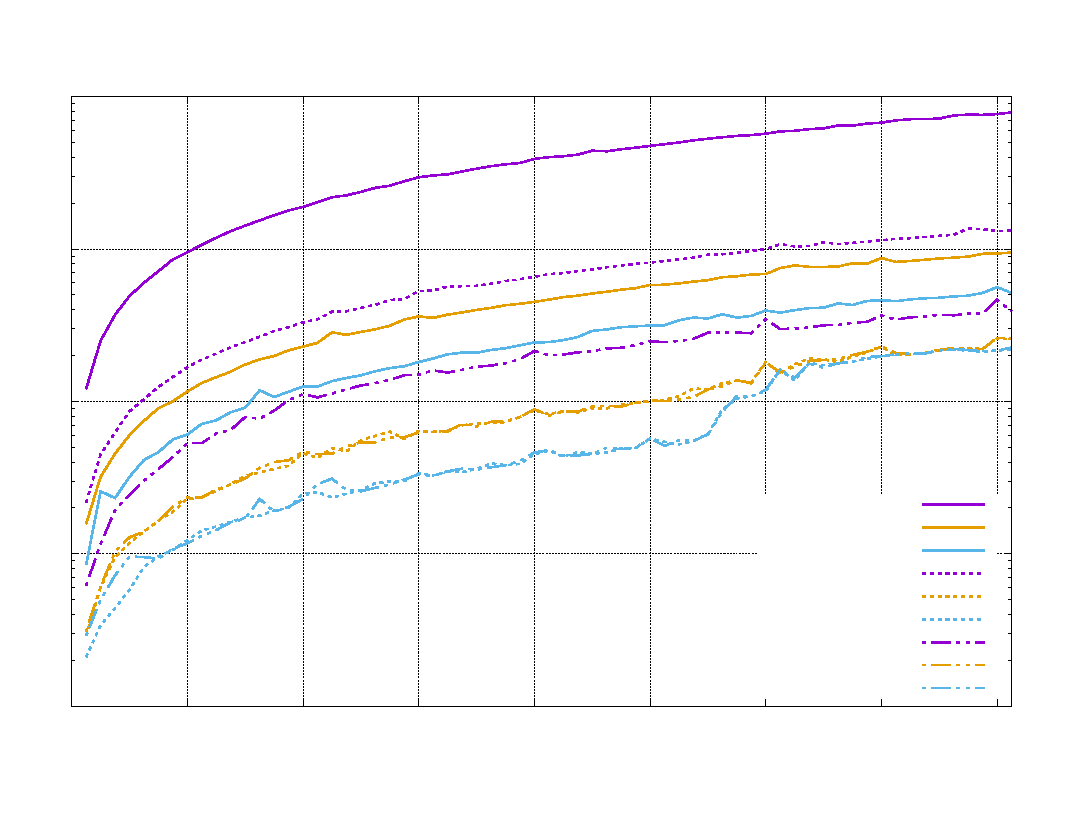
\includegraphics{scalar}}%
    \gplfronttext
  \end{picture}%
\endgroup
}
	\caption{Input dynamic range calculation.}
	\label{Fig:SCALAR}
\end{figure}
\\\\Another fact worth mentioning is the presence of weird spikes on the figure, noticeable in particular in \textit{O3 SSE4 CMPLX STRUCT} (solid orange line). These spikes can always be found at multiples of 1024 bytes. The root cause of this problem s related to cache size and associativity: cache miss phenomena is made worse when the data size is a multiple of CPU cache's critical stride. In such cases, known as super alignment, previously allocated cache elements are constantly evicted for new elements that share the same cache set and line.
\\\\The last comparison is done between the two complex multiplication algorithms. Programming without SIMD intrinsics does not provide competitive results against the handwritten SIMD functions. The speedup ratio is around 4x for SSE4 and 7x for AVX2 in with the struct function, while it is between 3x an 1.3x for SSE4 and between 6x and 2.3x in the array function. An overview of the comparison can be seen in Figure \ref{Fig:CMPLEX}.
It is also interesting to notice that with input size lower than 6144 bytes, the array approach is faster with respect to the struct counterpart, while after this point, the two perform approximately the same.

\begin{figure}
	\centering
	\resizebox{1.0\textwidth}{!}{% GNUPLOT: LaTeX picture with Postscript
\begingroup
  \makeatletter
  \providecommand\color[2][]{%
    \GenericError{(gnuplot) \space\space\space\@spaces}{%
      Package color not loaded in conjunction with
      terminal option `colourtext'%
    }{See the gnuplot documentation for explanation.%
    }{Either use 'blacktext' in gnuplot or load the package
      color.sty in LaTeX.}%
    \renewcommand\color[2][]{}%
  }%
  \providecommand\includegraphics[2][]{%
    \GenericError{(gnuplot) \space\space\space\@spaces}{%
      Package graphicx or graphics not loaded%
    }{See the gnuplot documentation for explanation.%
    }{The gnuplot epslatex terminal needs graphicx.sty or graphics.sty.}%
    \renewcommand\includegraphics[2][]{}%
  }%
  \providecommand\rotatebox[2]{#2}%
  \@ifundefined{ifGPcolor}{%
    \newif\ifGPcolor
    \GPcolortrue
  }{}%
  \@ifundefined{ifGPblacktext}{%
    \newif\ifGPblacktext
    \GPblacktextfalse
  }{}%
  % define a \g@addto@macro without @ in the name:
  \let\gplgaddtomacro\g@addto@macro
  % define empty templates for all commands taking text:
  \gdef\gplbacktext{}%
  \gdef\gplfronttext{}%
  \makeatother
  \ifGPblacktext
    % no textcolor at all
    \def\colorrgb#1{}%
    \def\colorgray#1{}%
  \else
    % gray or color?
    \ifGPcolor
      \def\colorrgb#1{\color[rgb]{#1}}%
      \def\colorgray#1{\color[gray]{#1}}%
      \expandafter\def\csname LTw\endcsname{\color{white}}%
      \expandafter\def\csname LTb\endcsname{\color{black}}%
      \expandafter\def\csname LTa\endcsname{\color{black}}%
      \expandafter\def\csname LT0\endcsname{\color[rgb]{1,0,0}}%
      \expandafter\def\csname LT1\endcsname{\color[rgb]{0,1,0}}%
      \expandafter\def\csname LT2\endcsname{\color[rgb]{0,0,1}}%
      \expandafter\def\csname LT3\endcsname{\color[rgb]{1,0,1}}%
      \expandafter\def\csname LT4\endcsname{\color[rgb]{0,1,1}}%
      \expandafter\def\csname LT5\endcsname{\color[rgb]{1,1,0}}%
      \expandafter\def\csname LT6\endcsname{\color[rgb]{0,0,0}}%
      \expandafter\def\csname LT7\endcsname{\color[rgb]{1,0.3,0}}%
      \expandafter\def\csname LT8\endcsname{\color[rgb]{0.5,0.5,0.5}}%
    \else
      % gray
      \def\colorrgb#1{\color{black}}%
      \def\colorgray#1{\color[gray]{#1}}%
      \expandafter\def\csname LTw\endcsname{\color{white}}%
      \expandafter\def\csname LTb\endcsname{\color{black}}%
      \expandafter\def\csname LTa\endcsname{\color{black}}%
      \expandafter\def\csname LT0\endcsname{\color{black}}%
      \expandafter\def\csname LT1\endcsname{\color{black}}%
      \expandafter\def\csname LT2\endcsname{\color{black}}%
      \expandafter\def\csname LT3\endcsname{\color{black}}%
      \expandafter\def\csname LT4\endcsname{\color{black}}%
      \expandafter\def\csname LT5\endcsname{\color{black}}%
      \expandafter\def\csname LT6\endcsname{\color{black}}%
      \expandafter\def\csname LT7\endcsname{\color{black}}%
      \expandafter\def\csname LT8\endcsname{\color{black}}%
    \fi
  \fi
    \setlength{\unitlength}{0.0500bp}%
    \ifx\gptboxheight\undefined%
      \newlength{\gptboxheight}%
      \newlength{\gptboxwidth}%
      \newsavebox{\gptboxtext}%
    \fi%
    \setlength{\fboxrule}{0.5pt}%
    \setlength{\fboxsep}{1pt}%
\begin{picture}(10080.00,7544.00)%
    \gplgaddtomacro\gplbacktext{%
      \csname LTb\endcsname%
      \put(396,924){\makebox(0,0)[r]{\strut{}\LARGE{$0$}}}%
      \csname LTb\endcsname%
      \put(396,2094){\makebox(0,0)[r]{\strut{}\LARGE{$2000$}}}%
      \csname LTb\endcsname%
      \put(396,3264){\makebox(0,0)[r]{\strut{}\LARGE{$4000$}}}%
      \csname LTb\endcsname%
      \put(396,4433){\makebox(0,0)[r]{\strut{}\LARGE{$6000$}}}%
      \csname LTb\endcsname%
      \put(396,5603){\makebox(0,0)[r]{\strut{}\LARGE{$8000$}}}%
      \csname LTb\endcsname%
      \put(396,6773){\makebox(0,0)[r]{\strut{}\LARGE{$10000$}}}%
      \csname LTb\endcsname%
      \put(528,594){\makebox(0,0){\strut{}\LARGE{$0$}}}%
      \csname LTb\endcsname%
      \put(1639,594){\makebox(0,0){\strut{}\LARGE{$1024$}}}%
      \csname LTb\endcsname%
      \put(2749,594){\makebox(0,0){\strut{}\LARGE{$2048$}}}%
      \csname LTb\endcsname%
      \put(3860,594){\makebox(0,0){\strut{}\LARGE{$3072$}}}%
      \csname LTb\endcsname%
      \put(4970,594){\makebox(0,0){\strut{}\LARGE{$4096$}}}%
      \csname LTb\endcsname%
      \put(6081,594){\makebox(0,0){\strut{}\LARGE{$5120$}}}%
      \csname LTb\endcsname%
      \put(7191,594){\makebox(0,0){\strut{}\LARGE{$6144$}}}%
      \csname LTb\endcsname%
      \put(8302,594){\makebox(0,0){\strut{}\LARGE{$7168$}}}%
      \csname LTb\endcsname%
      \put(9412,594){\makebox(0,0){\strut{}\LARGE{$8192$}}}%
    }%
    \gplgaddtomacro\gplfronttext{%
      \csname LTb\endcsname%
      \put(-638,3848){\rotatebox{-270}{\makebox(0,0){\strut{}\LARGE{clock cycles}}}}%
      \put(5039,154){\makebox(0,0){\strut{}\LARGE{input size [bytes]}}}%
      \put(5039,7213){\makebox(0,0){\strut{}\Large{\shortstack{Data Structure Comparison on 16-bit Fixed Point Complex Multiplication\\ O3 Optimization - Average on 500000 iterations}}}}%
      \csname LTb\endcsname%
      \put(3564,6600){\makebox(0,0)[r]{\strut{}\normalsize{O3 SCALAR CMPLX STRUCT}}}%
      \csname LTb\endcsname%
      \put(3564,6380){\makebox(0,0)[r]{\strut{}\normalsize{O3 SSE4 CMPLX STRUCT}}}%
      \csname LTb\endcsname%
      \put(3564,6160){\makebox(0,0)[r]{\strut{}\normalsize{O3 AVX2 CMPLX STRUCT}}}%
      \csname LTb\endcsname%
      \put(3564,5940){\makebox(0,0)[r]{\strut{}\normalsize{O3 SCALAR CMPLX ARRAY}}}%
      \csname LTb\endcsname%
      \put(3564,5720){\makebox(0,0)[r]{\strut{}\normalsize{O3 SSE4 CMPLX ARRAY}}}%
      \csname LTb\endcsname%
      \put(3564,5500){\makebox(0,0)[r]{\strut{}\normalsize{O3 AVX2 CMPLX ARRAY}}}%
    }%
    \gplbacktext
    \put(0,0){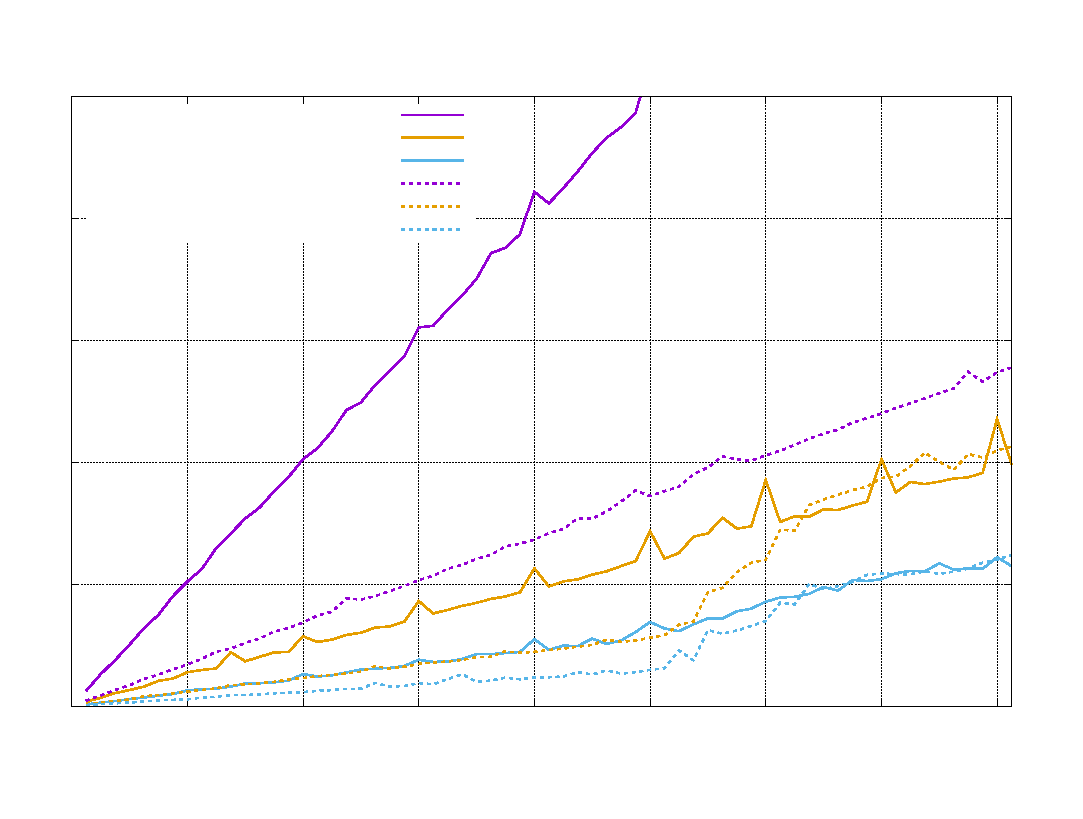
\includegraphics{complex}}%
    \gplfronttext
  \end{picture}%
\endgroup
}
	\caption{Input dynamic range calculation.}
	\label{Fig:CMPLEX}
\end{figure}

\clearpage
\printbibliography

\end{document}
